\documentclass[]{article}
\usepackage[margin=0.9in]{geometry}

\usepackage{enumitem}
\usepackage{graphicx}
\usepackage{hyperref}
\usepackage{float}
\usepackage{listings}
\lstset{
	language=bash,
	basicstyle=\ttfamily
}

\graphicspath{{images/test-policy-images/}}

\hypersetup{
	colorlinks=true,
	linkcolor=blue,
	filecolor=magenta,
	urlcolor=cyan,
}

%opening
\title{Testing Policy for Docks}
\author{TripleParity}
\date{}

\begin{document}

\maketitle

\tableofcontents

\section{Testing Process}
When a commit is made to the 'docks-ui' repository on GitHub two
processes are started:
\begin{itemize}
	\item \href{https://travis-ci.org/TripleParity/docks-ui/branches}{Travis CI} Builds the repository
	\item \href{https://hub.docker.com/r/tripleparity/docks-ui/builds/}{Docker Hub} builds the repository and creates a Docker Image that can be deployed in production
\end{itemize}

\subsection{Travis CI}
The history of test reports for Travis CI can be viewed at \url{https://travis-ci.org/TripleParity/docks-ui/branches}.
If the build was not successful it will be marked as 'failed'

\begin{figure}[H]
	\centering
	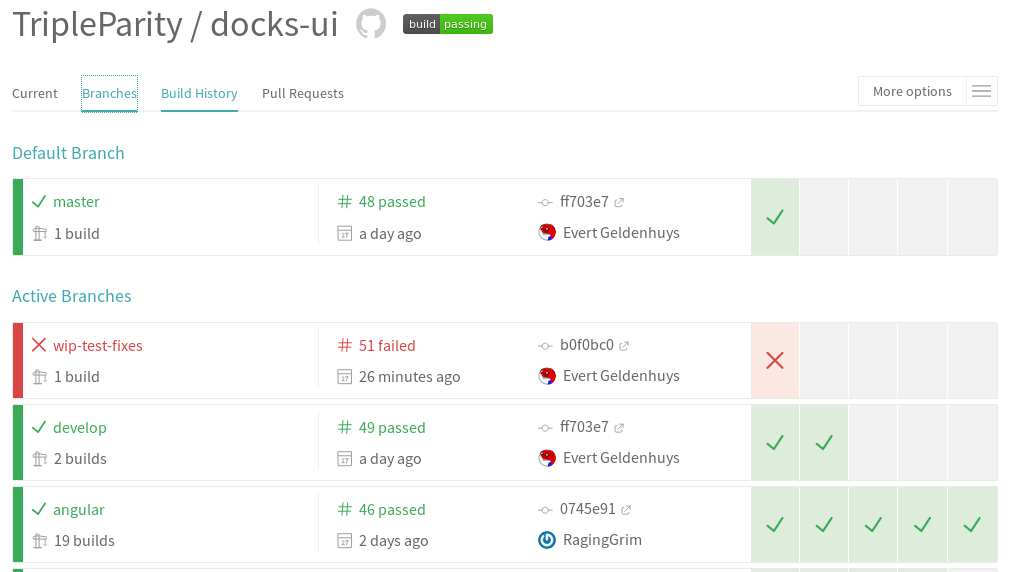
\includegraphics[scale=0.5]{test_travis_branches.png}
	\caption{Travis CI branch builds}
\end{figure}

\subsection{Docker Hub}
The history of builds for Docker Hub can be viewed at
\url{https://hub.docker.com/r/tripleparity/docks-ui/builds/}

\begin{figure}[h!]
	\centering
	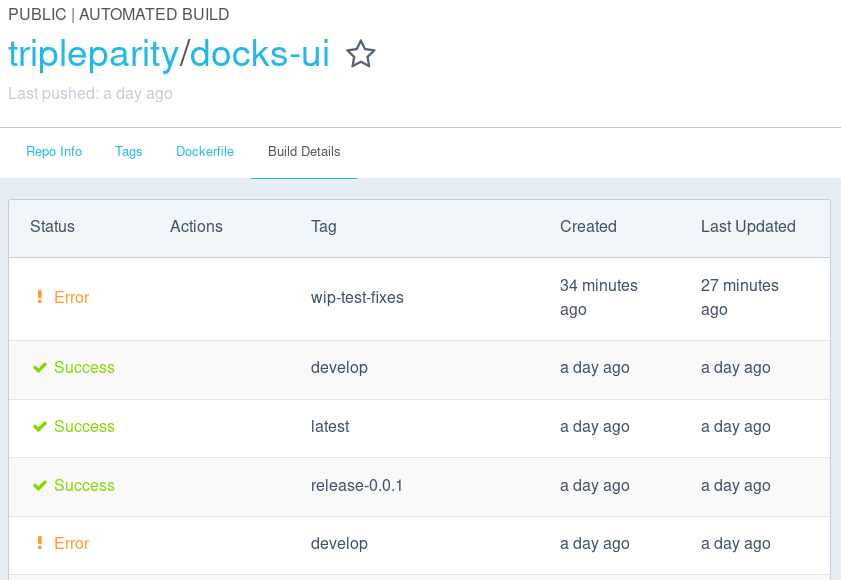
\includegraphics[scale=0.5]{test_docker_hub.png}
	\caption{Docker Hub builds}
\end{figure}

\end{document}
